\documentclass{../source/zju}

\articletitle{远程声控系统}
\major{信息工程}
\name{周灿松}
\stuid{3190105055}
\college{信息与电子工程学院}
\date{\today}
\course{信息、控制与计算}
\instructor{张朝阳}
\Abstract{本次大作业实现并模拟了一个远程声控系统,该系统一共可以接收十个指令,并可以通过这十个指令控制一个可控系统完成一定的动作。为了简化工作,我们在此假设了十个指令等概率发生,以此为基础生成了霍夫曼编码的码书。该系统工作原理如下:接收到语音输入后,将其量化,然后对其霍夫曼编码去冗余,随后利用卷积码进行信道编码;对其施加一个高斯白噪声信号模拟信道传输过程。接收端接收到信号解调后首先进行信道解码,然后信源解码,随后利用MATLAB预训练的语音CNN模型识别指令,打印出指令作为执行单元。}
\Keyword{远程声控、信源编码、信道编码、语音识别}

\begin{document}
    \makeheader
    \section{问题}
    实现一个远程声音控制系统。首先采集不同的语音指示信号,进行适当压缩;然后通过噪声信道实现远程传输,远端接收后再通过适当计算识别出是何指示,最后送入一个处于未知状态、但能控/能观的控制系统,完成不同的控制动作。

    \section{问题分析与解决思路}
    首先需要采集不同的语音指示信号,在这一步,我选择了使用MATLAB中的audiorecorder函数录制了时长为1秒的十个指令。信号传输部分,采用了如图\ref{信号传输模型}所示的信号传输模型,因为没有学习调制解调的相关知识,此处直接调用了MATLAB的pskmod函数实现了BPSK调制。将原始信号进行量化后,经过信源编码、信道编码、调制解调信道译码、信源译码得到传输后的信号。在信源编码部分,我采用了平均码字最短的霍夫曼码以获得较高的压缩率;信道编码部分采用了后续章节中的卷积码进行,以此提高信号传输的可靠性;传输过程中加入了高斯白噪声作为干扰信号模拟真实信道;语音识别部分则采用MATLAB预训练的语音识别模型来识别译码后的信号;执行部分为打印对应指令。

    \begin{figure}[H]
        \centering
        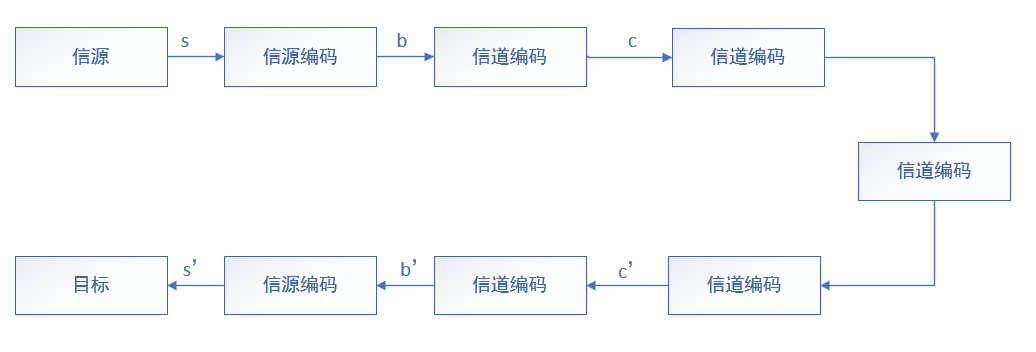
\includegraphics[width = \textwidth]{figure/信号传输mox.png}
        \caption{信号传输模型}
        \label{信号传输模型}
    \end{figure}

    \section{实现过程}
        \subsection{声音信号采集}
           麦克风的输入信号为幅值连续的模拟信号,在通信系统中,信息用01表示,所以我们必须将其转换为数字信号才能够在数字系统中进行应用,这一过程就涉及到了采样、量化与编码。

           此步骤对声音信号进行采样,在这一步中我调用了MATLAB中的audiorecorder函数录制麦克风的输入信号。设置采样率为8000Hz,采样位数为16位,单声道,录音时长1s。以stop信号为例,可以得到采样后的信号时域图与频域图如图\ref{sample}所示。

        \begin{figure}[H]
            \centering
            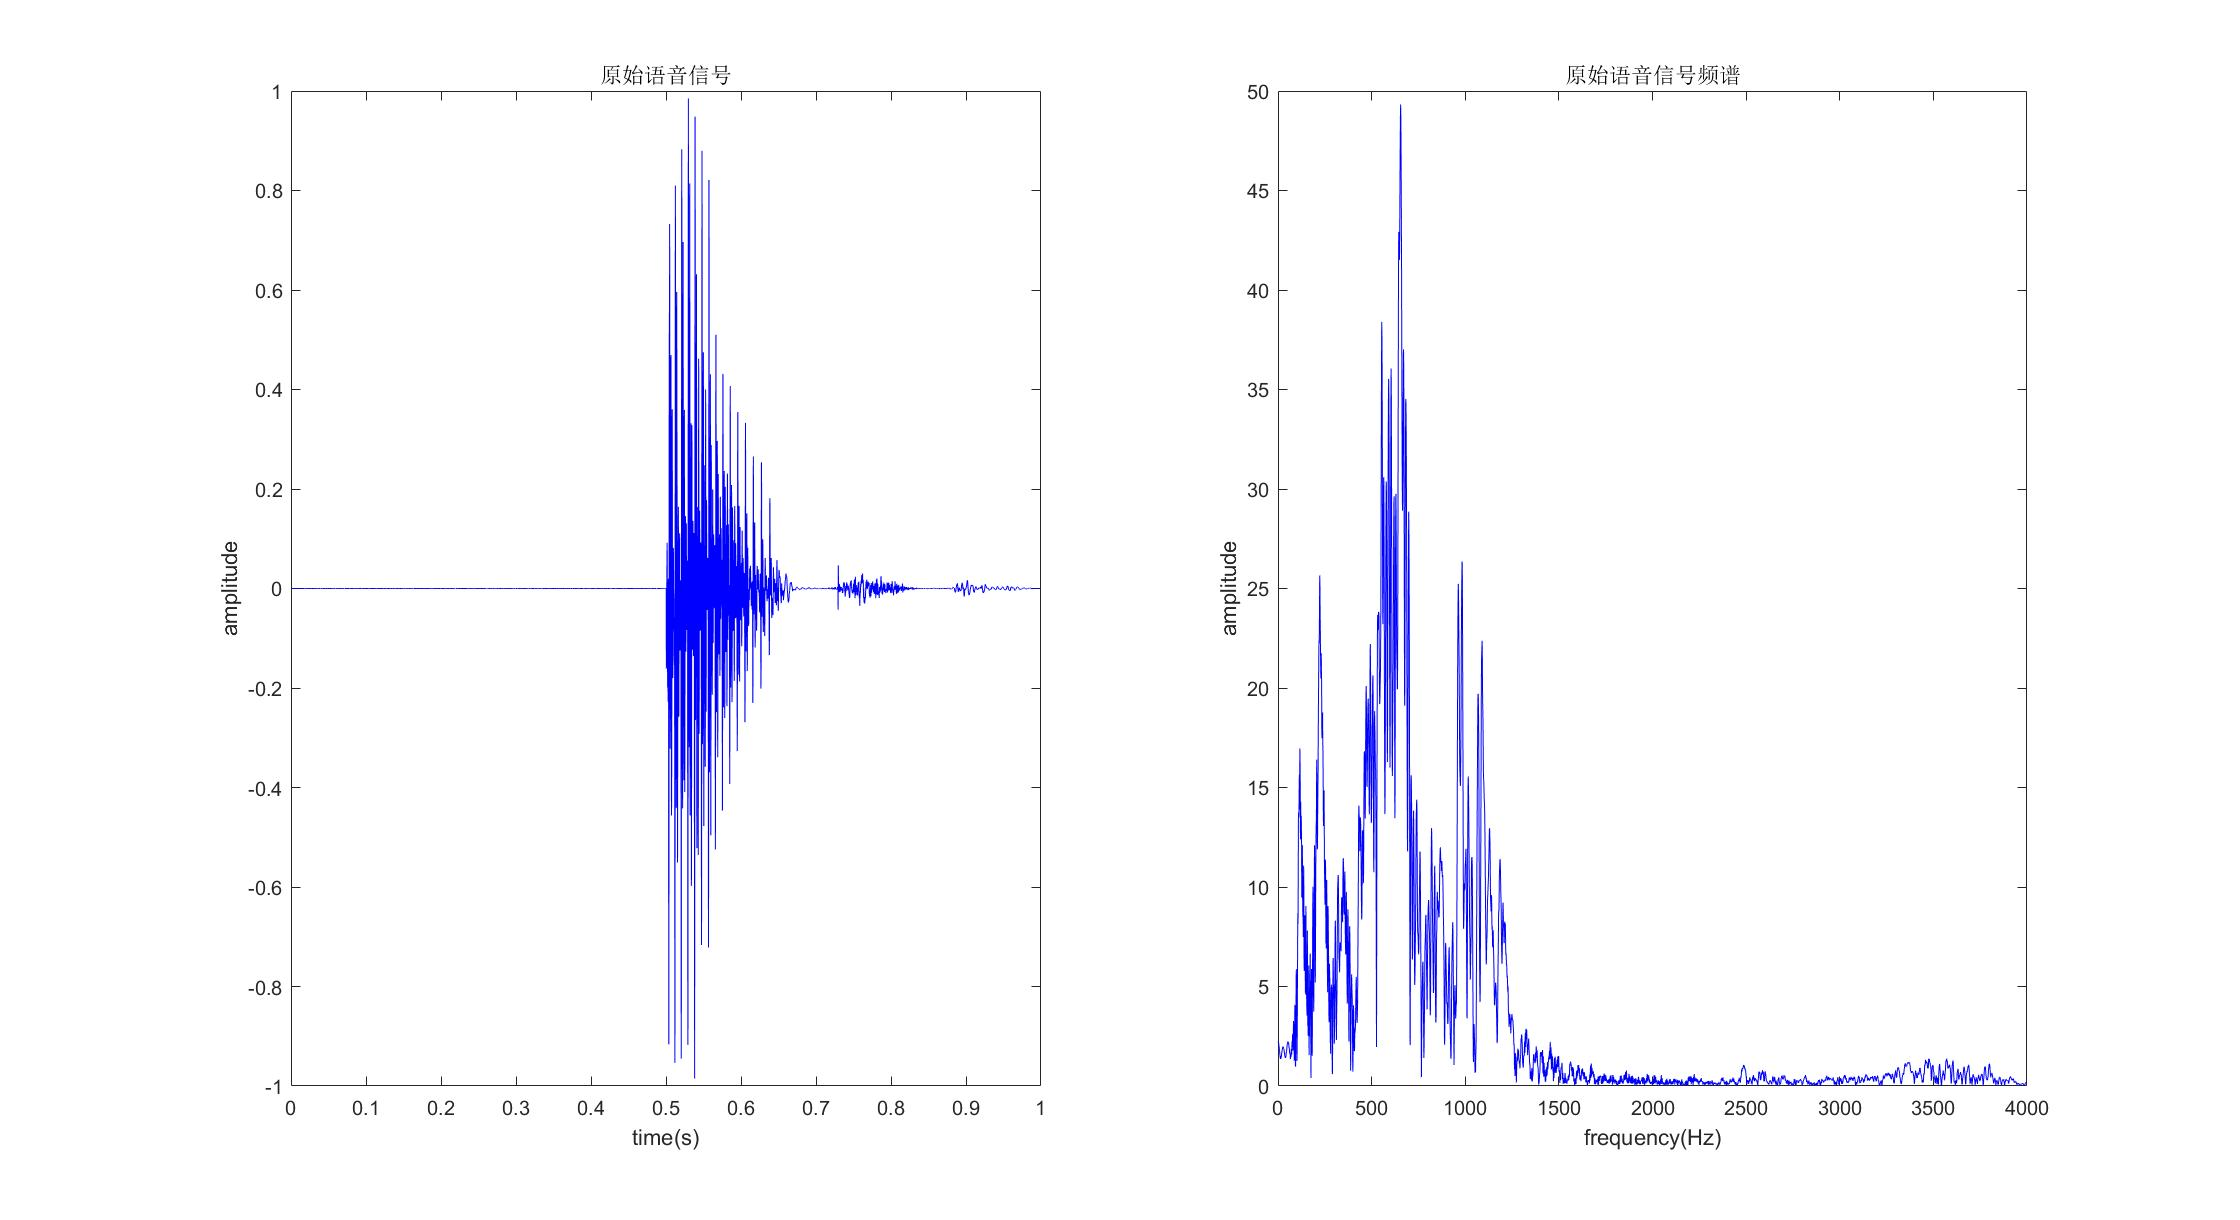
\includegraphics[width = \textwidth]{figure/sample.jpg}
            \caption{采样后的时域图与频域图}
            \label{sample}
        \end{figure}

        \subsection{量化以及编码}
        因为任何数字系统的存储都是有限的,所以我们需要对前面采样得到的信号进行量化以及编码,图\ref{量化示意}表达了[0,1],量化等级为3的二进制量化。
        \begin{figure}[H]
            \centering
            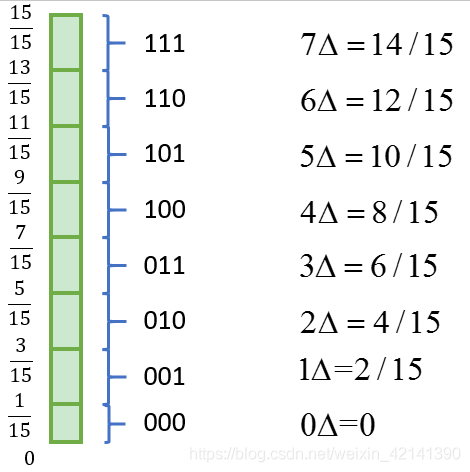
\includegraphics[scale = 0.3]{figure/量化示例.png}
            \caption{[0,1],量化等级为3的二进制量化}
            \label{量化示意}
        \end{figure}
        在本次作业中,我对[-1,1]采用了量化等级为8的二进制量化,量化器的分辨率为:
        $$q = \frac{1-(-1)}{2^N} = \frac{2}{2^8} = 7.8125\times10^{-3}$$
        量化后的声音时域图与量化前进行对比如图\ref{量化对比}所示
        \begin{figure}[H]
            \centering
            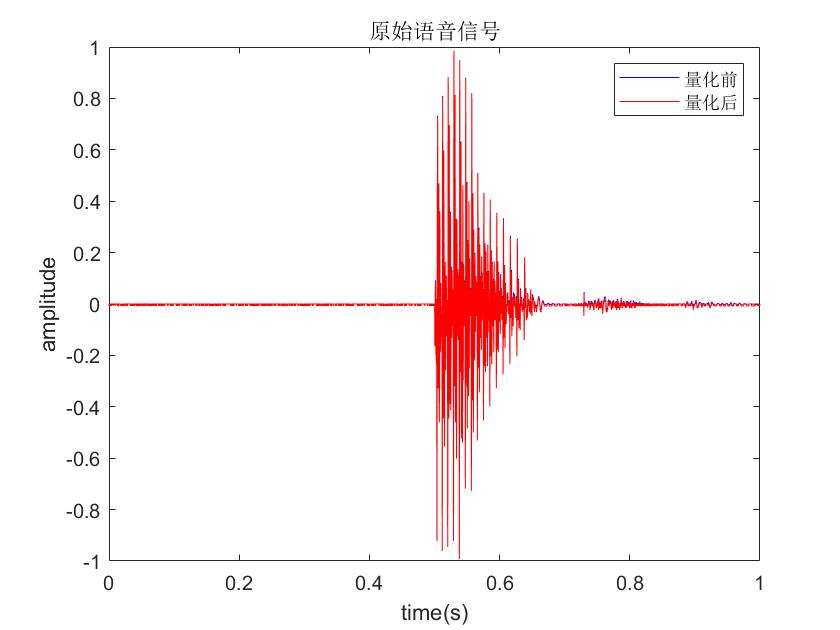
\includegraphics[scale = 0.3]{figure/量化后.jpg}
            \caption{量化前后声音信号对比}
            \label{量化对比}
        \end{figure}

        \subsection{生成码书}
        因为我们假设了十种指令等概率出现,所以我们在生成用于霍夫曼编码的码书时将十种指令各取一次合计算各个幅值出现的概率用于生成霍夫曼编码的码书。下面介绍霍夫曼编码的基本步骤:
            \begin{enumerate}
                \item 将信源符号按出现概率从大到小排列
                \item 将最小的两个概率相加,形成一个新概率
                \item 再将概率进行重新排列,如此重复直到只有两个概率为止
                \item 分配码字。码字分配从最后一步开始反方向进行,对最后两个概率一个赋予“0”码字,一个赋予“1”码字,如此反方向进行到开始的概率排列
            \end{enumerate}
        在本步骤中,我们先计算了各个符号出现的概率,然后调用了MATLAB中的huffmandict函数生成码书,图\ref{码书统计}展示了该码书的统计结果:平均码长为2.808909bit,因为为2元码,所以编码速率也为2.808909。同时可以看出信源熵为2.776450,可以看出编码速率大于信源熵,符合信源编码定理。并且可以计算出编码效率为0.988444。
        \begin{figure}[H]
            \centering
            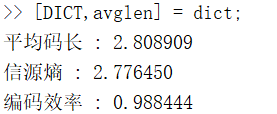
\includegraphics[]{figure/码书统计.png}
            \caption{码书统计结果}
            \label{码书统计}
        \end{figure}

        \subsection{信源编码}
        利用上一步生成的码书对量化后的序列进行编码,编码统计如图\ref{编码统计}所示,比起8bit量化的结果,霍夫曼编码的编码长度减小了一半多,压缩率达到了2.523062
        \begin{figure}[H]
            \centering
            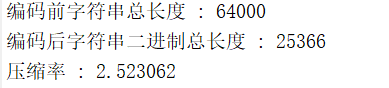
\includegraphics[]{figure/编码统计.png}
            \caption{编码统计结果}
            \label{编码统计}
        \end{figure}

        \subsection{信道编码}
        信道编码在对信源编码压缩后的数据加入了一定数量受到控制的冗余度,使得数据在传输过程或者接收过程中发生的差错可以被纠正或者发现,从而能够正确地恢复出原始数据信息。

        在本次作业中,我选择了课本后续章节会讲到的卷积码进行信源编码。与分组码不同,卷积码的编码器是有记忆性的。在任意给定时刻编码器的n个输出比特不仅和当前的k(bit)输入数据相关,而且和以前M个时刻的输入组相关,所以卷积码可以用(n,k,M)来描述。码率$R= \frac{k}{n}$。卷积码的编码过程示例如图\ref{卷积码示例}所示。
        \begin{figure}[H]
            \centering
            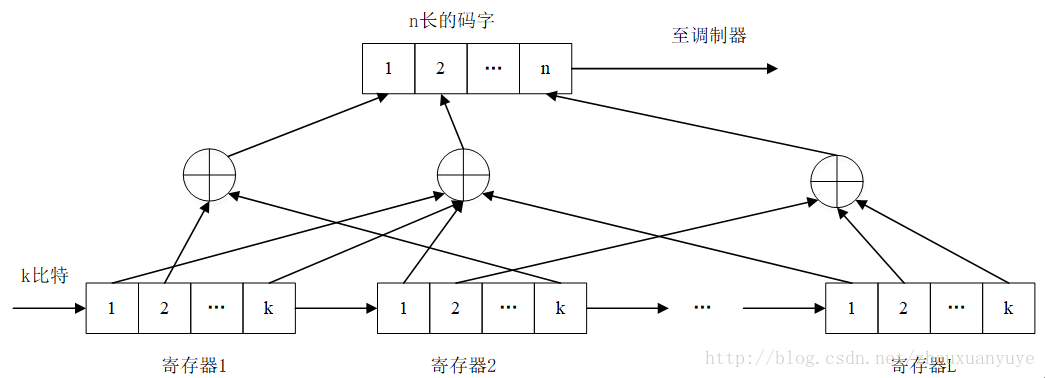
\includegraphics[width = \textwidth]{figure/卷积码示意图.png}
            \caption{卷积码示意图}
            \label{卷积码示例}
        \end{figure}
        我使用了MATLAB中的poly2trellis函数将(2,1,6)卷积码生成了MATLAB的网格表达式,随后利用convenc函数对输入序列进行了编码。在这一卷积码中,码率为$\frac{1}{2}$.

        信道编码结果如图\ref{信道编码结果}所示,计算所得码率为0.5,符合预期
        \begin{figure}[H]
            \centering
            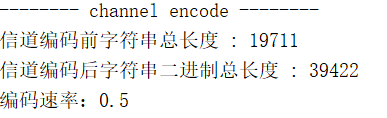
\includegraphics[]{figure/信道编码结果.png}
            \caption{信道编码结果}
            \label{信道编码结果}
        \end{figure}

        \subsection{调制解调}
        BPSK调制:二进制相移键控。是把模拟信号转换成数据值的转换方式之一,利用偏离相位的复数波浪组合来表现信息键控移相方式。BPSK使用了基准的正弦波和相位反转的波浪,使一方为0,另一方为1,从而可以同时传送接受2值(1比特)的信息。

        加性高斯白噪声(AWGN),加性指的是叠加在某信号上;高斯指的是概率分布里的正态分布函数,白噪声指的是它的二阶矩不相关,一阶矩为常数,是指先后信号在时间上的相关性。如果这个噪声的幅度服从高斯分布,功率谱密度又是均匀分布的,则称它为高斯白噪声。

        因为需要模拟信道传输过程,所以需要对信道编码后的结果进行调制。因为还未学习调制解调相关知识,所以在此调用了MATLAB的pskmod函数实现了BPSK调制。

        在调制之后,使用MATLAB的awgn函数为调制后的信号加入高斯白噪声,以此模拟真实信道传输。
        
        图\ref{接收信号}为通过信道传输后的结果。
        \begin{figure}[H]
            \centering
            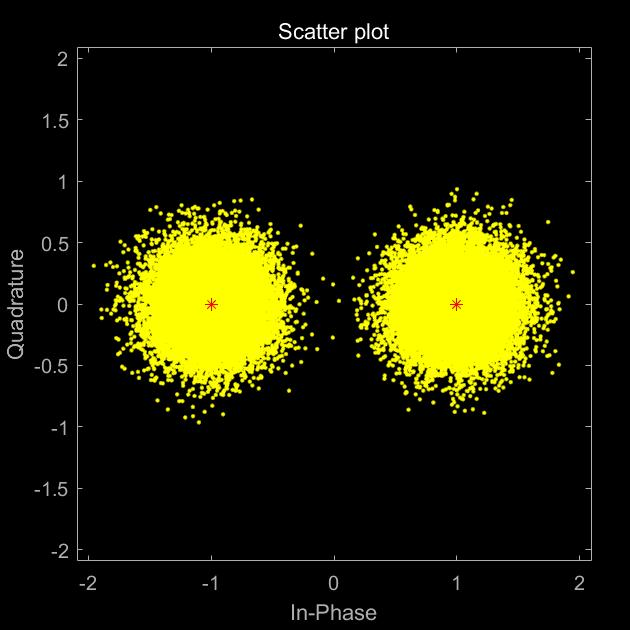
\includegraphics[scale = 0.4]{figure/接收信号.jpg}
            \caption{信道传输后信号}
            \label{接收信号}
        \end{figure}
        随后将该信号传入解调模块进行解调,在这一过程中,我测试了不同信噪比(-20dB~20dB)下调制解调的出错比特数以及出错率,结果如图\ref{解调统计}所示:随着SNR不断地提高,解调后信号的出错率逐渐降低,这是由于高斯白噪声信道的信道容量会随着信噪比的提高而提高。当SNR达到9左右时,解调的结果基本已经没有误差了。
        \begin{figure}[H]
            \centering
            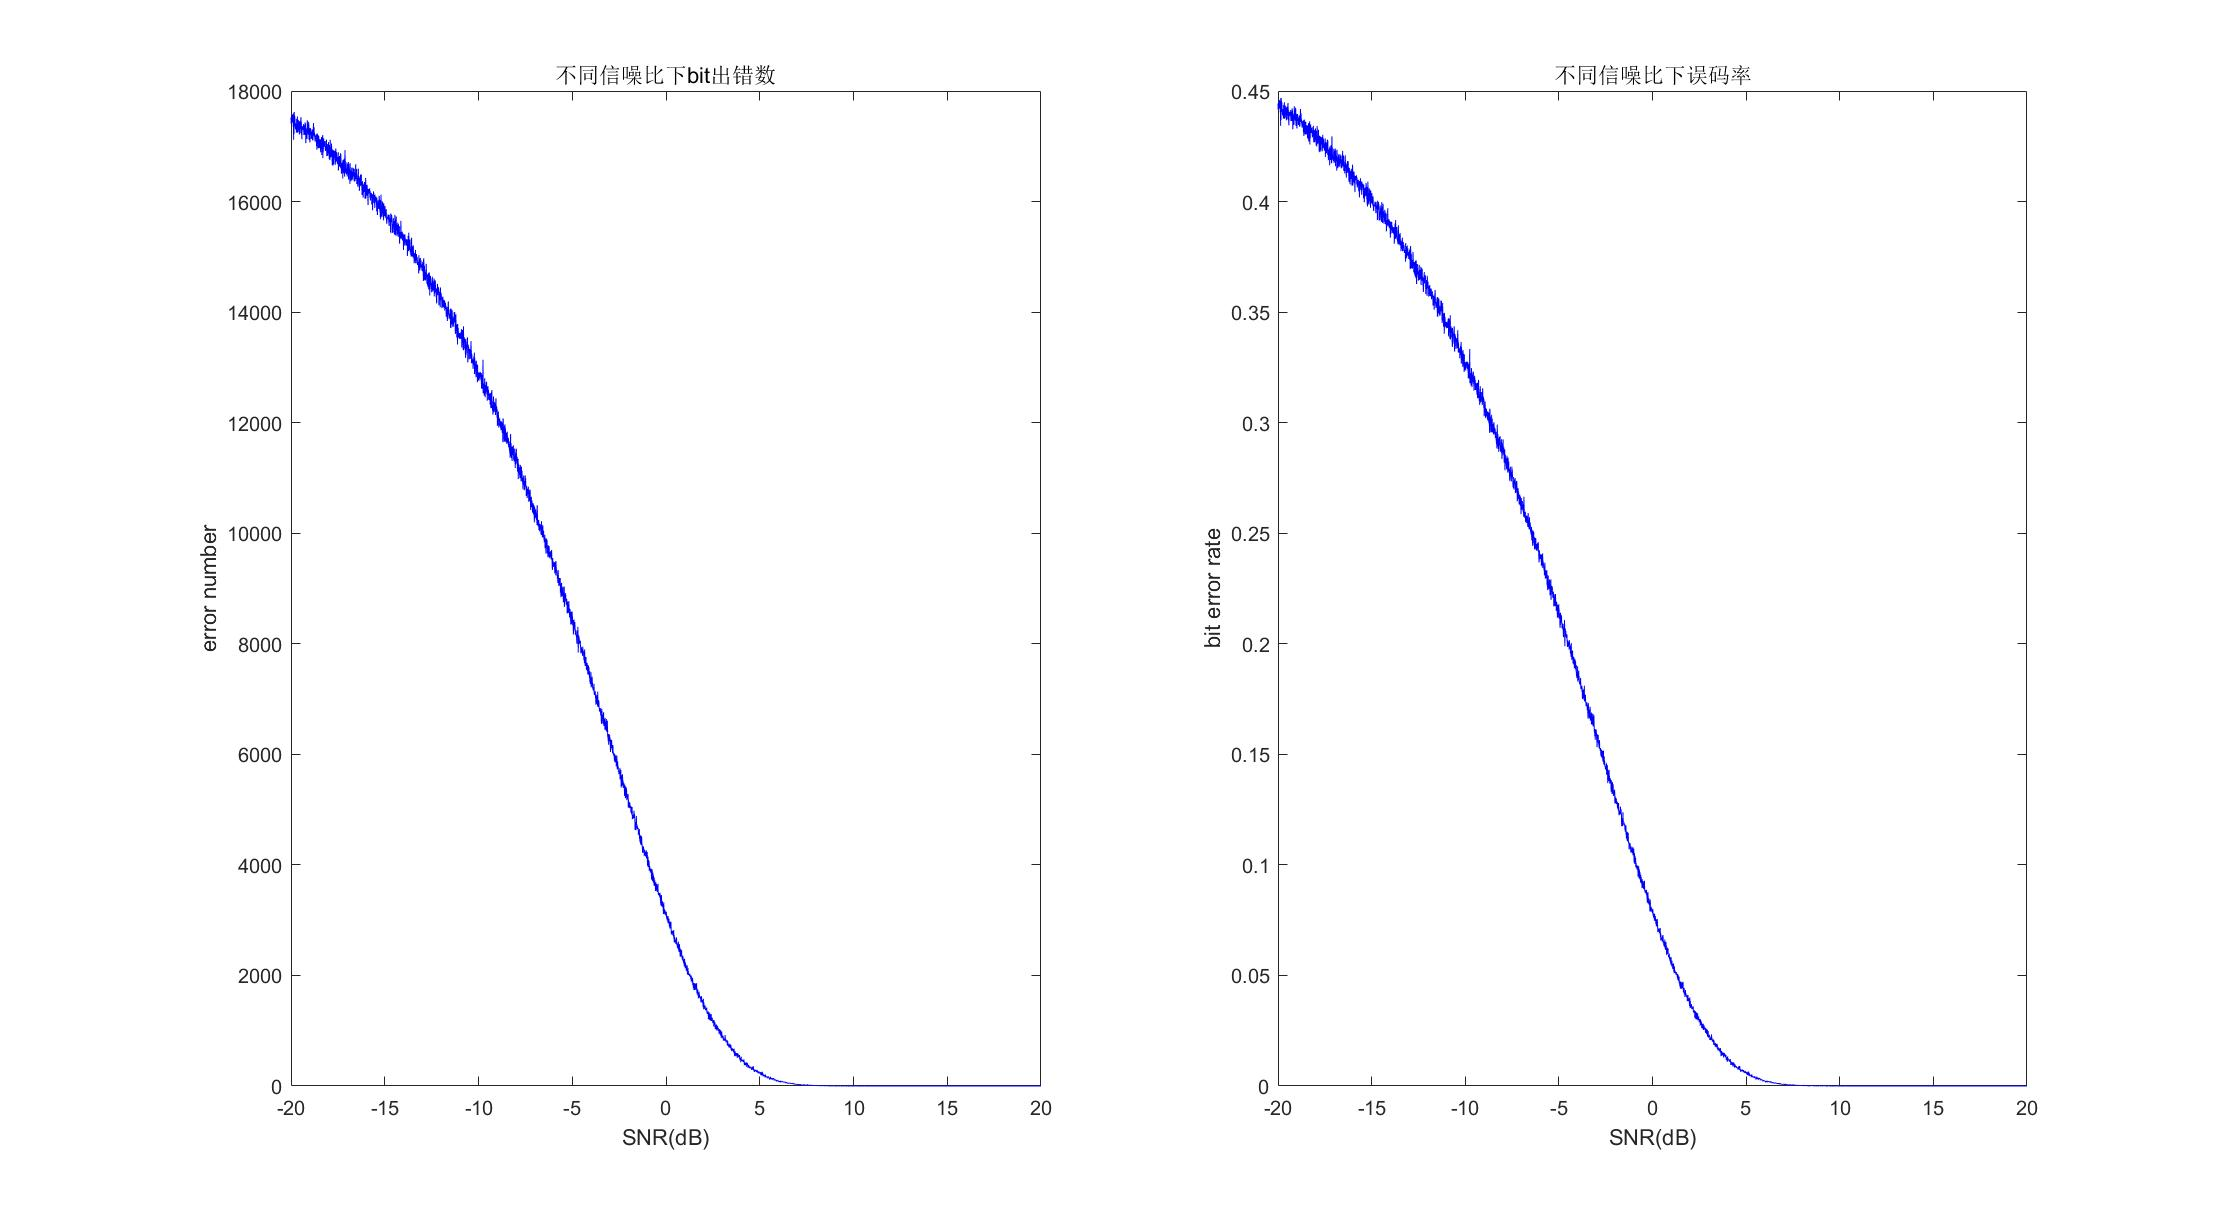
\includegraphics[width = 0.55\textwidth]{figure/解调结果.jpg}
            \caption{解调结果统计}
            \label{解调统计}
        \end{figure}

    \subsection{信道译码}
        因为在信道编码过程中使用了(2,1,6)卷积码进行编码,所以在此步需要用到卷积码的Viterbi译码算法进行信道译码。MATLAB中的vitdec函数能够实现这一目标。同样的,我测试了不同信噪比(-20dB~20dB)下信道译码的出错比特数以及出错率,如图\ref{信道解码}所示:与解调的结果类似,信道解码的出错率同样随着SNR的提高而降低,但不同的是,如果需要使信道解码达到无差错,SNR仅需要达到3左右即可,远远低于解调无差要求的9。这一点说明了信道编码解码的纠错作用是十分显著的。
        \begin{figure}[H]
            \centering
            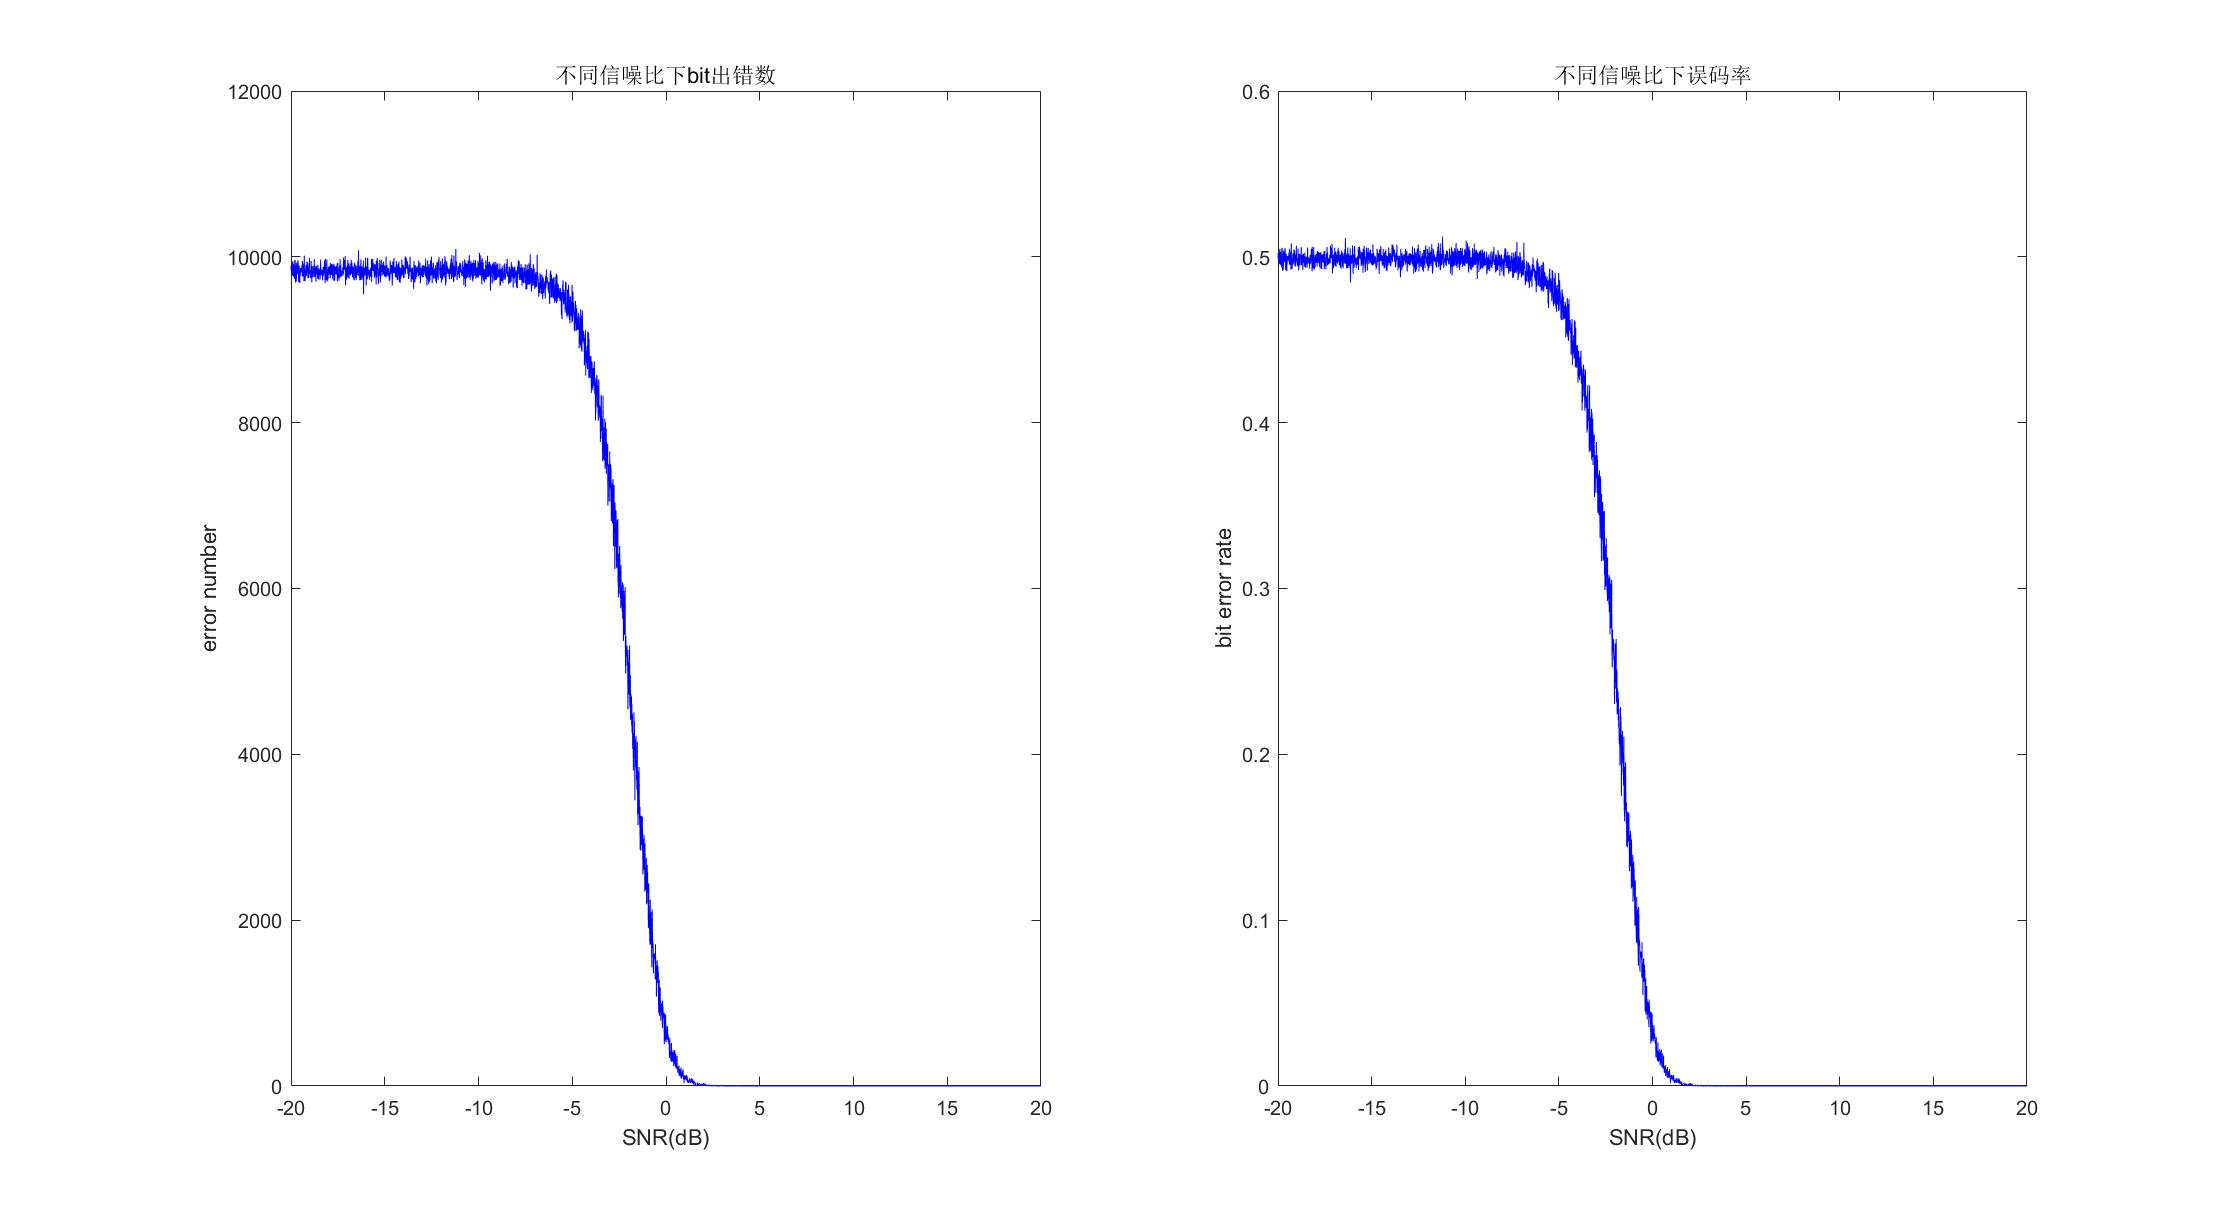
\includegraphics[width = 0.55\textwidth]{figure/信道解码.jpg}
            \caption{信道译码统计}
            \label{信道解码}
        \end{figure}

    \subsection{信源译码}
        得到信道译码的结果之后,我们需要进行信源译码以得到采样信号的量化值。因为信源编码时采用了霍夫曼编码,所以在此步也应当使用同一本码书进行信源译码。此步可以调用MATLAB中的huffmandeco函数实现,在SNR=10的情况下,译码出错比特以及出错率如图\ref{信源译码}所示。
        \begin{figure}[H]
            \centering
            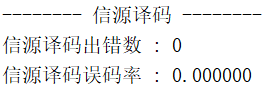
\includegraphics[]{figure/信源译码.png}
            \caption{信源译码统计}
            \label{信源译码}
        \end{figure}

    \subsection{信号重建}
        在量化阶段,我们将模拟信号量化为了0000\_0000--1111\_1111之间的离散信号,所以在接收端需要将信源译码得到的信号重新转换为模拟信号。

        重建后信号与原始信号的对比如图\ref{对比}所示。
        \begin{figure}[H]
            \centering
            \begin{minipage}[t]{0.48\textwidth}
            \centering
            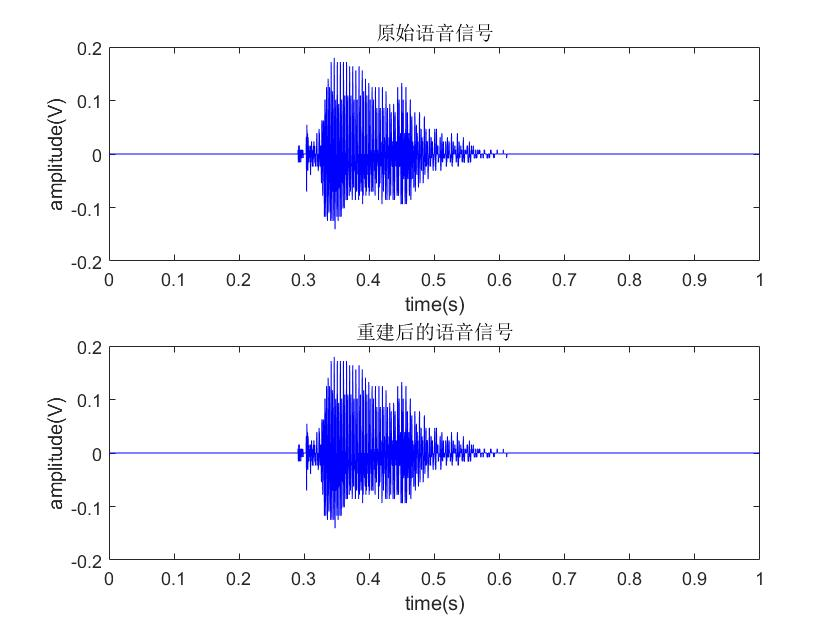
\includegraphics[width=\textwidth]{figure/时域对比.jpg}
            \end{minipage}
            \begin{minipage}[t]{0.48\textwidth}
            \centering
            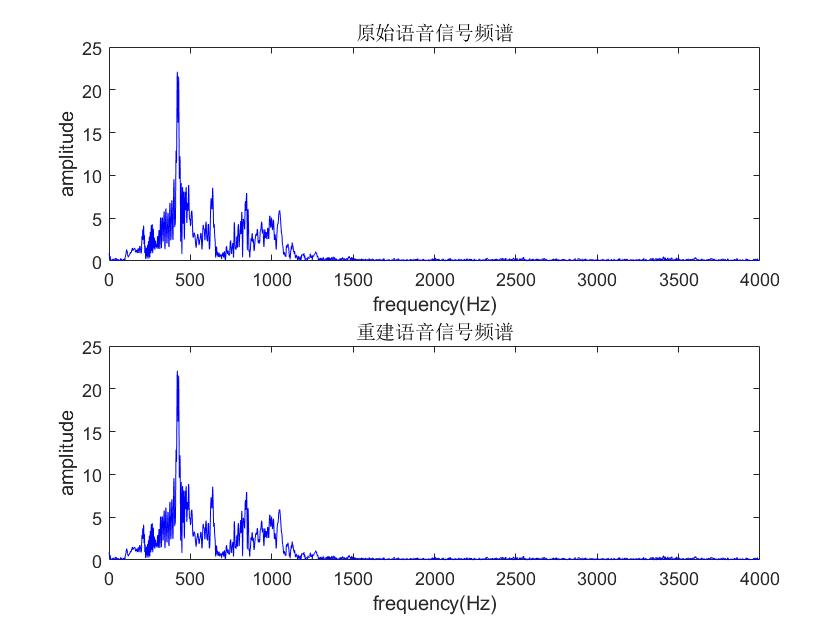
\includegraphics[width=\textwidth]{figure/频域对比.jpg}
            \end{minipage}
            \caption{重建前后对比}
            \label{对比}
        \end{figure}

    \subsection{语音识别}
        语音识别模块的作用是将重建得到的语音信号转换为对应的文本。在本设计中,我没有采用传统的HMM 声学模型而是使用了现下较为流行的CNN,利用卷积的不变性来克服语音信号本身的多样性。CNN 模型将整个语音信号分析得到的时频谱当作一张图像一样来处理,采用图像中广泛应用的深层卷积网络对其进行识别。

        为了节约训练成本,我利用了MATLAB预训练的语音CNN模型识别指令。可以识别”yes”,”no”,”up” ”down”,”left”,”right”,”on”,”off”,”stop”,”go” 共10 条指令,其余指令为unknown。

        语音识别模块的操作流程为:
        \begin{enumerate}
            \item 通过load函数导入预训练模型的参数。
            \item 通过helperExtractAuditoryFeatures 提取重新后语音信号的特征信息
            \item 通过classify 函数对声音的特征信息进行分类,输出分类后的指令信息。
        \end{enumerate}
        语音输出结果如图\ref{输出结果}所示。
        \begin{figure}[H]
            \centering
            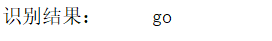
\includegraphics[]{figure/识别结果.png}
            \caption{识别结果}
            \label{识别结果}
        \end{figure}

    \subsection{动作控制}
        在这一部分,我假设了一个有限状态机作为被控模块,输入为上述十种指令,根据指令的不同以及当前状态决定下一状态,从而完成各种控制动作。在本次仿真中,由于没有相关材料,所以未实现本步,仅在此做阐释。

    \subsection{一次完整的指令传输过程}
        以go指令为例,图\ref{例子}展示了一次指令传输过程中的各种信息。
        \begin{figure}[H]
            \centering
            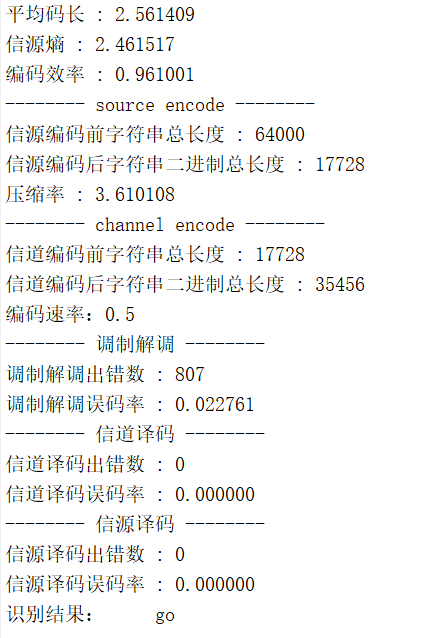
\includegraphics[]{figure/例子.png}
            \caption{go指令的传输}
            \label{例子}
        \end{figure}

\section{总结}
    在这次课程设计中,我利用MATLAB完成了一套远程语音控制系统的全过程仿真实现。
    
    首先是语音信号的采集部分,尤其需要注意将其进行合适的量化,只有在进行了量化之后才能够进入数字系统进行处理使用;
    
    然后在第二步的信源编码部分,选择了霍夫曼码对信源进行去冗余编码,由香农编码定理可知,在这个过程中需要注意编码速率必须大于信源熵才存在唯一可译的异字头码。在本次作业中,信源编码速率为2.808909,大于信源熵2.776450,所以是合理的。

    随后的信道编码则是为信息传输的可靠性打基础的步骤了。采用了码率为1/2的卷积码进行信道编码,由上文的分析也可以看出,信道编码将无损传输时所需要的信噪比由9dB降到了3dB左右,显著地提高了整个系统的可靠性。

    调制解调部分由于还没有学习相关的知识,在了解了调制解调的相关知识后直接调用了MATLAB中的相关函数实现。

    作业中的信道选择了加性高斯白噪声信道,由香农带限高斯信道容量公式可以发现该信道的容量与传输时的信噪比成正相关关系,所以能够通过提高信噪比减少传输误差的效果。

    通过这一次的大作业,我对信息、控制与计算这一门课上学到的知识有了更为深刻的认识,它将这门课上学到的各种知识有机地联系在了一起,各个知识点不再像以往一样分散在各个角落,互相有了联系,使得我的脑海里有了一个更加具体的知识图谱。
\end{document}